% Document information
% ====================
\title{Informe de práctica II}
\author{Dietrich Daroch}
\date{\normalsize\today}



% Document configuration
% ======================

% Document Type, Font and paper size
\documentclass[12pt, letterpaper]{article}

% Page Margins
\usepackage{fullpage}
\usepackage[top=4cm, left=4cm, bottom=2.5cm, right=2.5cm]{geometry}

% Text Margins
\setlength{\parindent}{0.49cm}
\renewcommand{\baselinestretch}{1.5}

% Font Type
%\usepackage{pslatex} %Times font
%\usepackage[font={small,sf},format=plain,labelfont=up]{caption}
\usepackage{helvet}
\renewcommand{\familydefault}{\sfdefault}

%% Languages
\usepackage[utf8]{inputenc}
\usepackage[british, spanish]{babel}

%% Basic imports
\usepackage{natbib}
\usepackage{graphicx}

%% Include PDF pages
\usepackage[final]{pdfpages}

%% Hyperlinks
\usepackage[pdfborder={0 0 0}]{hyperref} % no border

%% Math
\usepackage{amsmath}

%% Images
\DeclareGraphicsExtensions{.pdf,.png,.jpg}
\graphicspath{{graphics/}{images/}}
\usepackage{float}

%% Figure numbering
\usepackage{chngcntr}
\counterwithin{figure}{section}


%% Avoid Hyphens. Comment this code if you want to keep them.
\tolerance=1
\emergencystretch=\maxdimen
\hyphenpenalty=10000
\hbadness=10000

% Document text
% =============
\begin{document}
% Front
% -----
\includepdf[pages=-]{docs/cert.pdf}
\includepdf[pages=-]{docs/front.pdf}


% Evaluations
% -----------
% 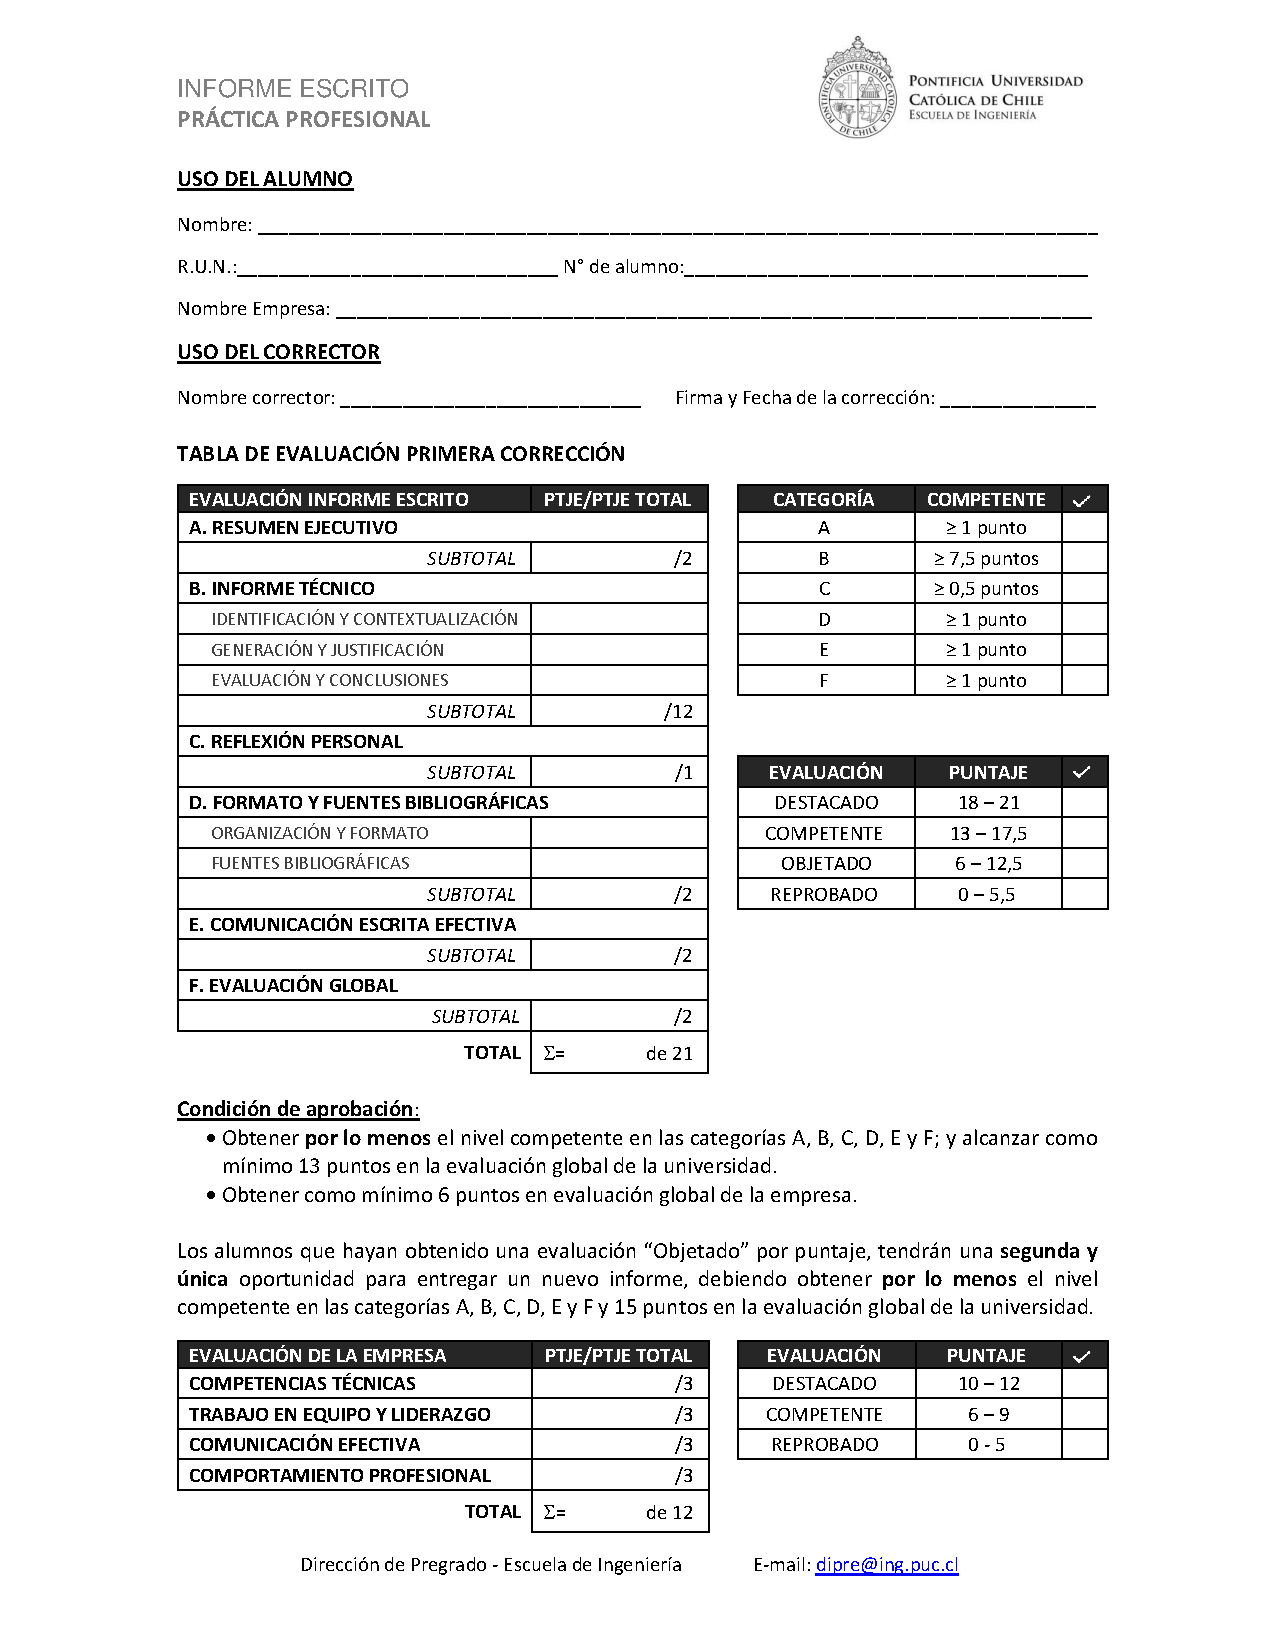
\includepdf[pages=-]{docs/university-evaluation.pdf}
% \includepdf[pages=-]{docs/internship-evaluation.pdf}


% Abstract
% --------
\pagenumbering{gobble}% Remove page numbers (and reset to 1)
% Resumen ejecutivo en inglés (Máximo una página)
% ===========================
%
% -Contextualiza el lugar de práctica (empresa, área) y el objetivo esperado al finalizar la práctica profesional.
% -Describe las principales actividades realizadas y las conclusiones del informe técnico.
% -Emplea un correcto uso de inglés cuidando la redacción y aspectos formales de la escritura (redacción (pls xd), ortografía y vocabulario).
\section*{Abstract}
\selectlanguage{british} % write like a sir
This is the abstract of my paper.
\newpage

\section*{Resumen ejecutivo}
\selectlanguage{spanish}
En este informe se comenta acerca de como se perdió un verano completo solo para rellenar este informe.
  % Abstract


% Indexes
% -------
\pagenumbering{arabic}% Arabic page numbers (and reset to 1)
\include{1-index}
% Informe técnico (Máximo 20 páginas)
% ===============
\section{Reporte técnico}

% Identificación y contextualización
% ----------------------------------
% - Contextualiza, en no más de una plana, el lugar de práctica (e.g: características de la empresa, área, tamaño de la empresa en relación al rubro, etc.)
% - Describe el proyecto en el cual se desempeñó el alumno (e.g: objetivo general, plazos, alcance, descripción técnica, etc.) y/o los principales procesos y agentes involucrados en el desarrollo de las actividades realizadas).
% - Identifica el objetivo o interés específico de la empresa a ser logrado durante la práctica y plantea un problema o pregunta a ser resuelto.
 
% - Detalla los antecedentes y causas del problema o pregunta planteada, e indica la importancia de su resolución.

\subsection{La empresa}
% \paragraph{}
La empresa “Neolítica SpA” (en adelante Neolítica) fue constituida en noviembre de 2018 por la colaboración entre 4 socios y la empresa Extend Comunicaciones S.A. (en adelante Extend), a raíz del interés del equipo de "Soluciones Educativas Educalabs Ltda" de cambiar de rumbo y formar un emprendimiento en desarrollo de software e inteligencia artificial. En el proceso apareció el proceso modernización de Extend, en el que estaban en busca de un emprendimiento de las mismas características en la que puedan invertir para que les desarrollen productos basados en inteligencia artificial, que mejores los servicios que ya ofrecen, además de que la empresa pueda vender otros servicios no necesariamente ligados a las necesidades de Extend, con el fin de que Neolítica crezca. Para hacer esto posible, y dentro del trato, Extend se comprometió a financiar a Neolítica durante un año, desde noviembre 2018 a noviembre 2019.
El equipo de desarrollo se compone de los cuatros socios naturales de la empresa, compuesto por tres estudiantes de ingeniería en computación y un estudiante de diseño, mientras que la administración y gerencia de Neolítica corre por cuenta de Extend como persona jurídica, también socia de la empresa.
El lugar de trabajo y oficina de Neolítica es en Rosario Norte 555, piso 12, en las dependencias de Extend, en un espacio exclusivo para la empresa otorgado tras el trato entre ambas empresas.

\subsection{El proyecto}

El proyecto a realizar corresponde al primer proyecto del emprendimiento, el cual nace a partir de uno de los servicios más vendidos dentro de Extend, el servicio de \textit{clipping}. Este consiste en realizar un compilado y resumen de las noticias de un período de tiempo (diario, semanal o mensual), para luego ser enviado al cliente que lo solicita, ya sea en períodos de campañas de prensa, como en períodos de crisis para la empresa. Estas noticias actualmente son recibidas desde proveedores de \textit{clippings}, los cuales recopilan noticias de distintos medios, los que luego clasifican automáticamente para que los periodistas de Extend puedan revisarlos y modificar el \textit{clipping} recibido si es necesario.

\subsection{Antecedentes del problema}

El problema detectado es que la calidad de estas recopilaciones enviadas desde los proveedores es muy baja, muchas veces con noticias de medios poco relevantes o que a veces no tienen relación alguna con el cliente. Esto produce que los periodistas deban eliminar muchas noticias y buscar otras para reemplazar, o simplemente realizarlo todo a mano. Esto produce un alto costo en tiempo para los periodistas y un gasto significativo en un servicio que no ofrece la calidad necesaria.
La información obtenida del problema fue levantada entrevistando a los propios periodistas encargados de estas tareas y algunos de los clientes de Extend.

\subsection{Objetivos de la empresa}

El objetivo de Neolítica es el de crear soluciones que puedan mejorar procesos a través del uso de inteligencia artificial y generar productos que permitan que el emprendimiento crezca y se pueda sustentar por sí solo una vez finalizado el financiamiento de la empresa Extend.
En específico para el proyecto, el objetivo es de implementar algoritmos que mejoren la selección de noticias, identifiquen las entidades presentes en una noticia, realicen un análisis sentimental respecto de cada entidad y en general, provea una plataforma amigable e intuitiva para poder preparar y enviar el \textit{clipping} en el mismo software. Como objetivo final, la empresa espera contar con una plataforma capaz de recolectar y almacenar una gran cantidad de datos (\textit{big data}) para poder obtener  nuevas conclusiones que permitan mejorar más el servicio de recomendación y reconocimiento de noticias y sus entidades.




% Generación y justificación
% --------------------------
% - Propone una metodología, herramientas y/o modelos para el análisis, diseño, desarrollo y solución del objetivo/problema (utiliza supuestos si no fueron aplicados durante el periodo de práctica).
   
 
% - Describe los análisis, mediciones o aplicaciones y los softwares necesarios para la resolución del problema/demanda (utiliza supuestos si no fueron aplicados durante el periodo de práctica).
   
 
% - Justifica las decisiones tomadas en cuanto a la metodología o los recursos utilizados de acuerdo a las características del problema/objetivo abordado y del lugar de realización de la práctica.
   
 
% - Utiliza recursos (e.g: como diagramas de flujo, figuras, gráficos, tablas, etc.) que facilitan el entendimiento de las labores realizadas o metodologías utilizadas


\subsection{Metodología y herramientas}

Para el desarrollo del proyecto, se implementó la metodología Scrum, la que fue utilizada en cursos como Ingeniería de Software, Desarrollo de Software y Proyecto de Especialidad, y que es conocida en el ámbito del software por ser una metodología ágil basada en iteraciones por períodos de tiempo. La forma de implementarla fue utilizando el libro Scrum and XP from the trenches, mismo libro sugerido y utilizado en el curso Desarrollo de Software, el cual se utilizó como referencia para realizar las distintas reuniones de trabajo: \textit{daily scrum}, \textit{sprint review} y \textit{sprint retrospective}. Cada iteración de desarrollo consistió en 4 semanas de desarrollo. Para cada una de estas iteraciones se eligieron los requisitos del software a realizar, se calculan las horas y luego las tareas son asignadas entre los miembros del equipo.
Se sugirió implementar el modelo \textit{PMBOK} (\textit{project management book of knowledge}), basado en los contenidos del curso Gestión de Proyectos de Tecnologías de la Información, para el desarrollo de la documentación del proyecto en sus distintas etapas: inicio, planificación, ejecución, monitoreo y control y cierre. Durante el período de práctica se desarrollaron los documentos de la fase de inicio y planificación, ya que el proyecto aún sigue en desarrollo.

\subsection{Solución propuesta}

Para desarrollar la solución del problema se propuso desarrollar una plataforma web, similar a la que utilizan actualmente en Extend para recibir clippings, pero con mejoras en los criterios de selección de la calidad de las noticias, a través de algoritmos de aprendizaje de máquina. El proyecto en su totalidad se compone de cinco entregables: una plataforma web gráfica (front-end), una API (application programming interface) con la que se comunica la plataforma web, una interfaz de desarrollo para acceder a la base de datos, un módulo de inteligencia artificial en el que se procesan los textos de noticias obtenidos y un módulo de obtención de noticias automatizado.

\subsection{Desarrollo de la solución}

\subsubsection{Levantamiento de requisitos}

El levantamiento de requisitos

\subsubsection{Elaboración de historias de usuario}

\subsubsection{Modelación, arquitectura e historias técnicas}

\subsubsection{Elección de tecnologías}

Para el desarrollo del software se tuvo que decidir por las tecnologías a utilizar, de manera que estas solucionaran el problema de la manera más óptima posible, considerando el estado del arte actual en desarrollo web, \textit{machine learning}, sistema de gestión de bases de datos y métodos de integración y despliegue contínuo. 
Para esto se decidió utilizar el lenguaje Python para los componentes que utilizan algoritmos de aprendizaje de máquina, dado su buen desempeño en tareas que requieren alto nivel de cómputo y la extensa comunidad de desarrolladores que contribuyen a la mejora de librerías de codigo abierto especialistas en aprendizaje de máquina. Por otraparte se escogió el lenguaje Javascript sobre el framework Node.JS para el desarrollo de las aplicaciones web, tanto \textit{frontend} como \textit{backend}, dada la capacidad de resistir múltiples usuarios recurrentes dado su funcionamiento asíncrono. En particular, el backend web utiliza el framework KOA, en conjunto con ...
Luego de la decisión de tecnologías se realizó un levantamiento de requisitos con los principales actores que participan del desarrollo de los clippings dentro de Extend.

\subsubsection{}

\subsubsection{\textit{Sprint Planning}}

\subsubsection{\textit{Sprint review} y \textit{sprint retrospective}}

\subsubsection{Producto Minimo Viable (\textit{MVP})}


% Conclusión
% ----------
%  Concluye los resultados, incluyendo: limitaciones y relevancia de los
%         análisis obtenidos; las implicancias futuras de las decisiones tomadas
%         y se discuten eventuales modificaciones y pasos a seguir.
\subsection{Conclusión}



% References
% ----------
\renewcommand\bibsection{\section{\refname}}
\bibliographystyle{alpha}
\bibliography{references}


% Appendix
% --------
\newpage
\section{Anexos}
\input{3-essay}

\newpage
% \includepdf[pages=-]{docs/log.pdf}

% Acá colocar todo el resto de los anexos

% \subsection{Diagrama de clases}

\end{document}
